\documentclass[11pt]{article}
\usepackage{geometry}                % See geometry.pdf to learn the layout options. There are lots.
\geometry{letterpaper}                   % ... or a4paper or a5paper or ... 
%\geometry{landscape}                % Activate for for rotated page geometry
\usepackage[parfill]{parskip}    % Activate to begin paragraphs with an empty line rather than an indent
\usepackage{graphicx}
\usepackage{amssymb}
\usepackage{epstopdf}
\usepackage{lscape}
\usepackage{hyperref}

\usepackage{changebar}
% disable display of changebars
%\nochangebars

% make figure and table captions narrower than the full page
\usepackage{caption}
\captionsetup{width=0.8\textwidth}


\DeclareGraphicsRule{.tif}{png}{.png}{`convert #1 `dirname #1`/`basename #1 .tif`.png}

% common header content elements
\title{Observations About OpenLCB CAN Timing}
\author{Bob Jacobsen}
\date{May 26, 2024}                                         % Activate to display a given date or no date

\begin{document}
\maketitle

% to format XML tags in proper angle brackets <>
\newcommand*{\xml}[1]{\texttt{<#1>}}

\newcommand{\ts}{\textsuperscript}

\newcommand{\us}{$\mu$s}

\section{Introduction}

There have been some recent discussions of whether the OpenLCB Standards
should, or even can, require that the frames of a message be sent 
sequentially on the CAN bus. This would be particularly important
for the proposed Event-with-Payload protocol update.

This note describes measurements of the OpenLCB CAN timing of 
a TCS CS-105 command station,
JMRI PanelPro connected via an LCC-Buffer USB, 
an RR-Cirkits Tower-LCC,
and an SPROG DCC Ltd. SERVOIO-LCC
to try to shed some light on 
current behavior in this 
area.\footnote{
The original version of this note was dated March 24, 2024. This
version includes an update, marked by change bars, to the new
version 1.5 of the SPROG SERVO-IO firmware.
}

\section{Measurement Setup}

The measurement setup consisted of a single CAN segment using 6" cables connecting, 
in order:
\begin{enumerate}
\item An RR-CirKits terminator.
\item An RR-Cirkits LCC Buffer-USB connected to a 2021 M1 Mac PowerBook Pro running 
    OlcbChecker\footnote{Available on 
                \href{http://github.com/bobjacobsen/OlcbChecker}{GitHub}. }
    for stimulating the device being measured.
\item A second RR-Cirkits LCC Buffer-USB connected to that same Powerbook Pro running 
    JMRI PanelPro 5.7.5 to log the bus traffic.
\item An XDS3104E digital storage oscilloscope attached to the CAN+ and CAN- lines.
    The scope signal ground is isolated from power ground and attached to CAN signal ground.
\item An RR-CirKits Power Point with a 15V power supply.
\item The device being measured.
\item An RR-CirKits CAN terminator.
\end{enumerate}

All stimuli were sent from a suitably-modified version of
OlcbChecker’s signal\_generator script
running on the PowerBook Pro.  
The Mac was idle except for running JMRI and the OlcbChecker script.  

We use the following bit notation when measuring the time between frames:\footnote{Figure from 
\href{https://en.wikipedia.org/wiki/CAN_bus}{Wikipedia}. }
\begin{figure}[!htbp]
\centering
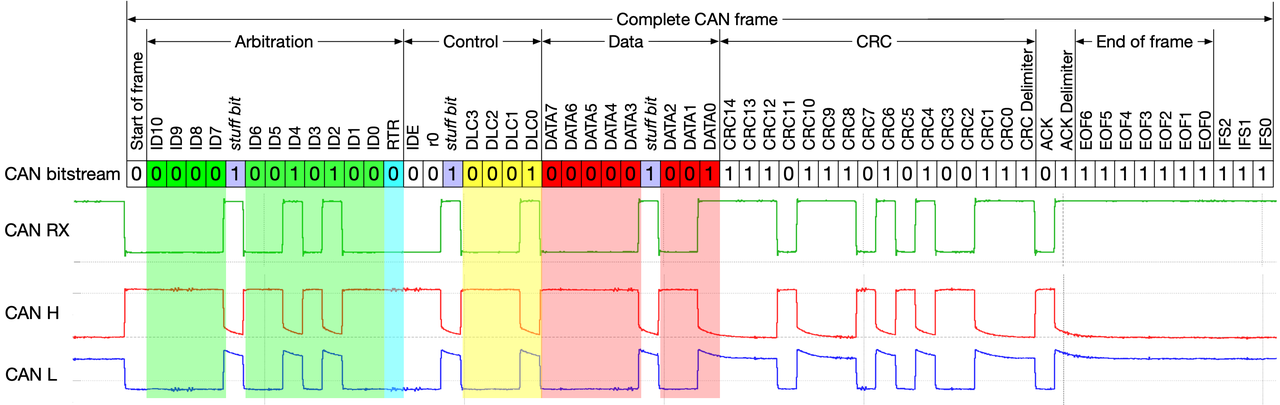
\includegraphics[width=1.0\linewidth]{CAN-bus-frame}
\caption{CAN Frame Notation}
\label{fig:CAN_frame}
\end{figure}

What we call ``the interframe time" is determined
by measuring from the trailing edge of an ACK bit
to the leading edge of the next Start of Frame bit and then subtracting the 
CAN protocol minimum of
11 bit times or 88 microseconds.
The interframe time will be zero if the frames follow each other sequentially. 

\subsection{Limitations}
The setup described here has some limitations:
\begin{enumerate}
\item It's not practical to decode individual packets on the scope.  That's done 
    using the JMRI monitor.
\item The JMRI monitor screen's timing display is not sufficiently precise
    for measuring the time of arrival of CAN frames. 
    It's only used to record the order of arrival of the frames and to decode their contents.
\item The scope has limited dynamic range on the horizontal axis.  Measurements of 
    the overall timing of a sequence have to be made in separate shots from
    the measurement of e.g. individual CAN frame timing.
\end{enumerate}

\section{Devices Being Measured}

\subsection{TCS CS-105}

This self-identifies as hardware version Rev E
and software version 1.00

\subsection{RR-CirKits Tower-LCC}

This self-identifies as hardware version rev-D
and software version rev-C7e.

\subsection{JMRI PanelPro}

JMRI release 5.7.4 was running on the slowest machine I have, a 2017 3GHZ iMac.  
It was connected to the OpenLCB CAN bus using an LCC Buffer-USB.

\subsection{SPROG DCC Ltd. SERVOIO-LCC}

\cbstart
This self-identifies as hardware version 1.0
and software version 1.5.
\cbend
\section{Measurements}

\subsection{Single SNIP Interaction}

This measurement sends a single SNIP request and examines the timing of the reply.
A typical interaction is shown in Figure \ref{fig:single_CS105_SNIP_interaction}.
Figure \ref{fig:single_CS105_SNIP_interframe} shows more detail of the time
between the first and second frames within the reply.

\begin{center}
\begin{tabular}{| l |c | c |}
\hline
Device &  Typical Reply Time & Typical Interframe Time\\
\hline
CS-105   &  10 ms & 0\us \\
JMRI   &  1.2 ms & 0\us \\
Tower-LCC   &  0.4 ms & 12 - 20 \us \\
\cbstart SERVOIO-LCC   &  0.6-1.0 ms & 0\us \cbend \\
\hline
\end{tabular}
\end{center}

To summarize, all four devices have enough delay 
between receiving a request and sending the response
for another packet to be put on the CAN bus. 
\cbstart
The CS-105, JMRI and SERVIO-LCC
reply without inter-frame delays while the Tower-LCC
has an additional delay between reply frames that would
allow a lower-priority frame to be inserted.
\cbend

\begin{figure}[!htbp]
\centering
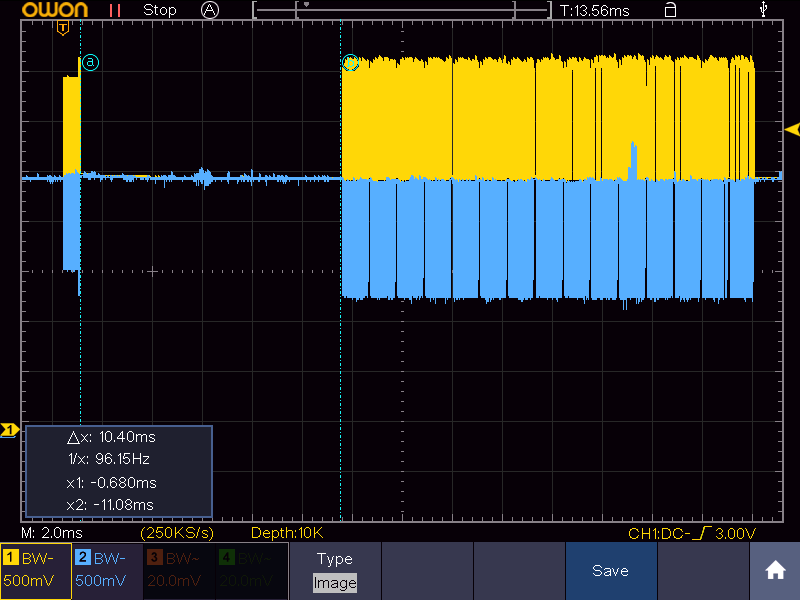
\includegraphics[width=1.0\linewidth]{1SNIP_CS105_Full}
\caption{Overview of a single CS105 SNIP interaction. 
The first frame on the left is the SNIP request message.
The SNIP reply message is made up of the 15 frames in the middle.}
\label{fig:single_CS105_SNIP_interaction}
\end{figure}

\begin{figure}[!htbp]
\centering
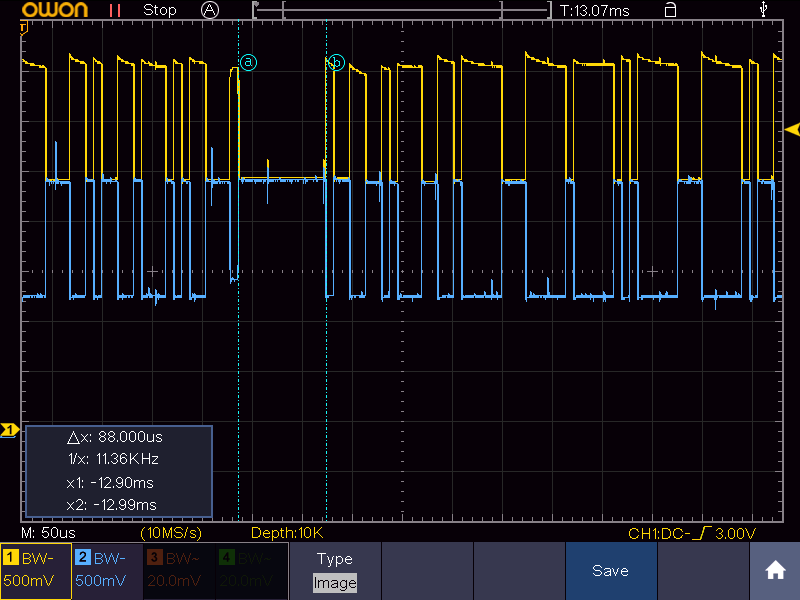
\includegraphics[width=1.0\linewidth]{1SNIP_CS105_Spacing}
\caption{Interframe delay of CS105 SNIP reply. 
The time cursors are on the trailing edge of the first reply frame's ACK bit 
and the leading edge of the next Start of Frame bit.}
\label{fig:single_CS105_SNIP_interframe}
\end{figure}


\begin{figure}[!htbp]
\centering
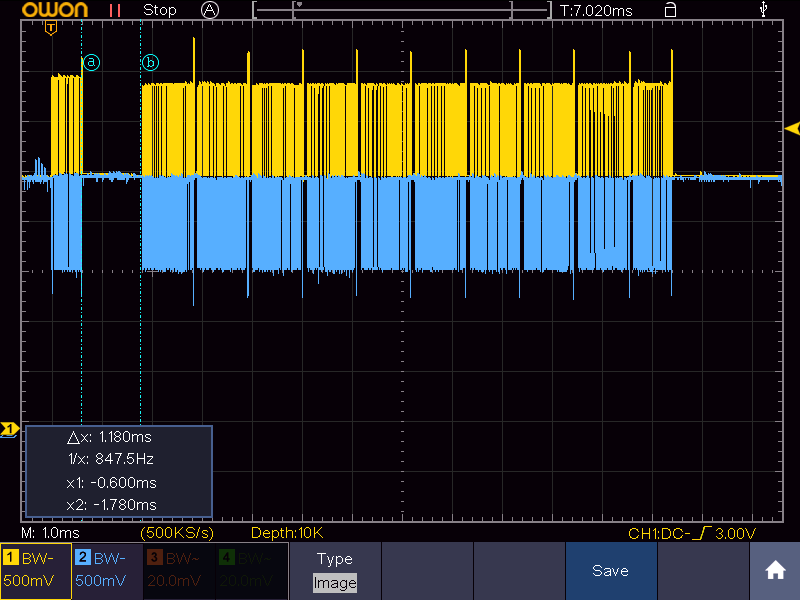
\includegraphics[width=1.0\linewidth]{1SNIP_JMRI_Full}
\caption{Overview of a single JMRI SNIP interaction.}
\label{fig:single_JMRI_SNIP_interaction}
\end{figure}

\begin{figure}[!htbp]
\centering
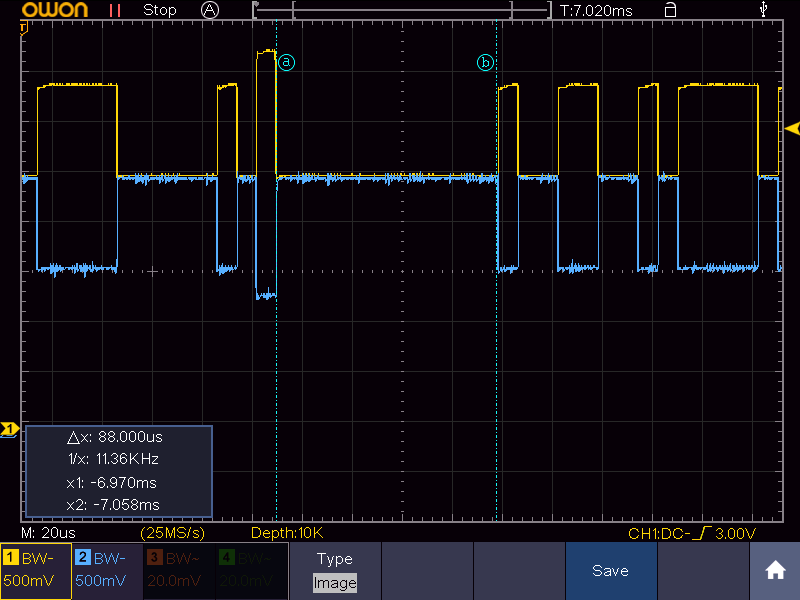
\includegraphics[width=1.0\linewidth]{1SNIP_JMRI_Spacing}
\caption{Interframe delay of JMRI SNIP reply.}
\label{fig:single_JMRI_SNIP_interframe}
\end{figure}


\begin{figure}[!htbp]
\centering
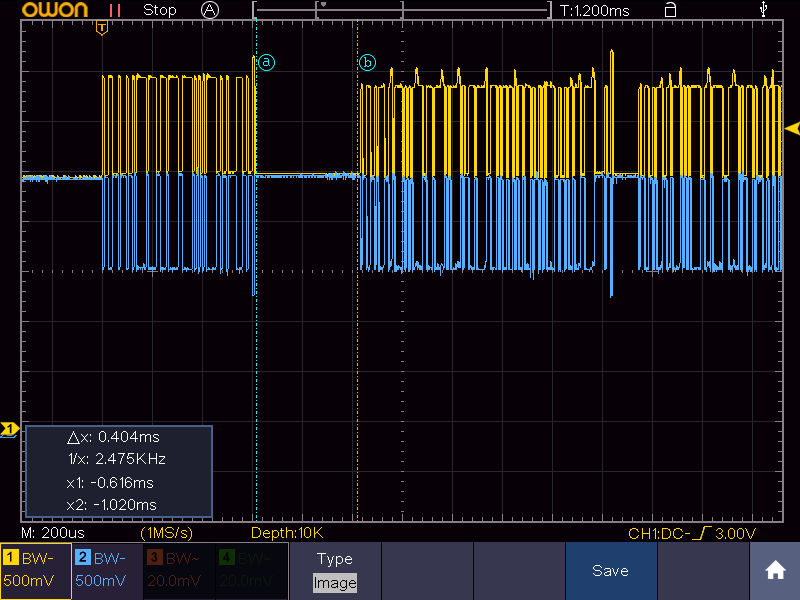
\includegraphics[width=1.0\linewidth]{1SNIP_TWR_Delay}
\caption{View of a single Tower-LCC SNIP interaction
showing the initial reply time.
The entire set of reply frames is not shown to get additional
precision on the reply time measurement.}
\label{fig:single_TWR_SNIP_interaction}
\end{figure}

\begin{figure}[!htbp]
\centering
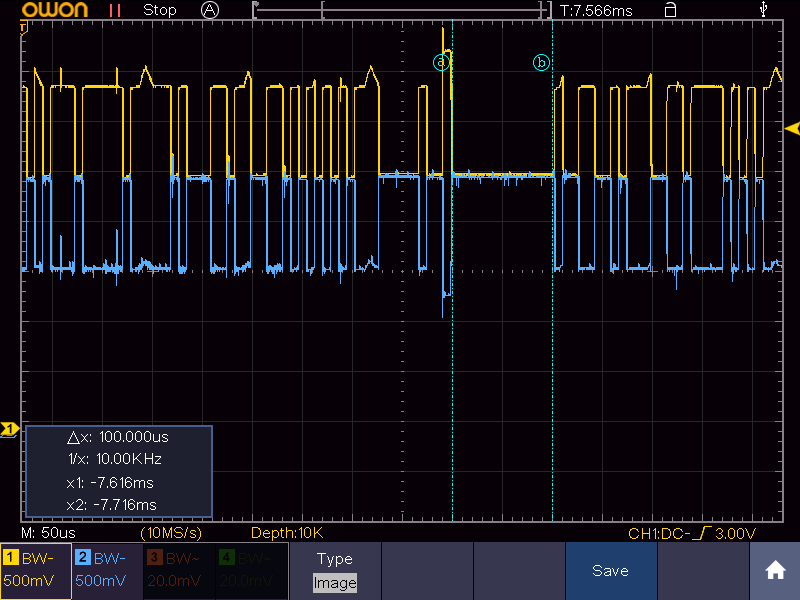
\includegraphics[width=1.0\linewidth]{1SNIP_TWR_Spacing}
\caption{Interframe delay of Tower-LCC SNIP reply.
After the required 88 \us, there's an additional 12\us 
inter-frame delay.}
\label{fig:single_TWR_SNIP_interframe}
\end{figure}


\cbstart
\begin{figure}[!htbp]
\centering
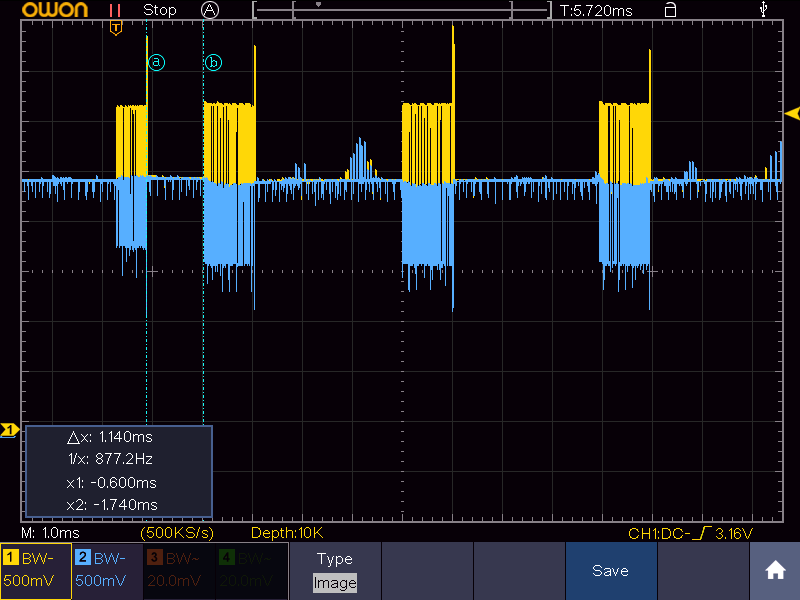
\includegraphics[width=1.0\linewidth]{1SNIP_SPROG_Start_delay_1_140}
\caption{Overview of a single SERVOIO-LCC SNIP interaction.
The entire set of reply frames is not shown to get additional
precision on the reply time measurement.}
\label{fig:single_SERVOIO_SNIP_interaction}
\end{figure}

\begin{figure}[!htbp]
\centering
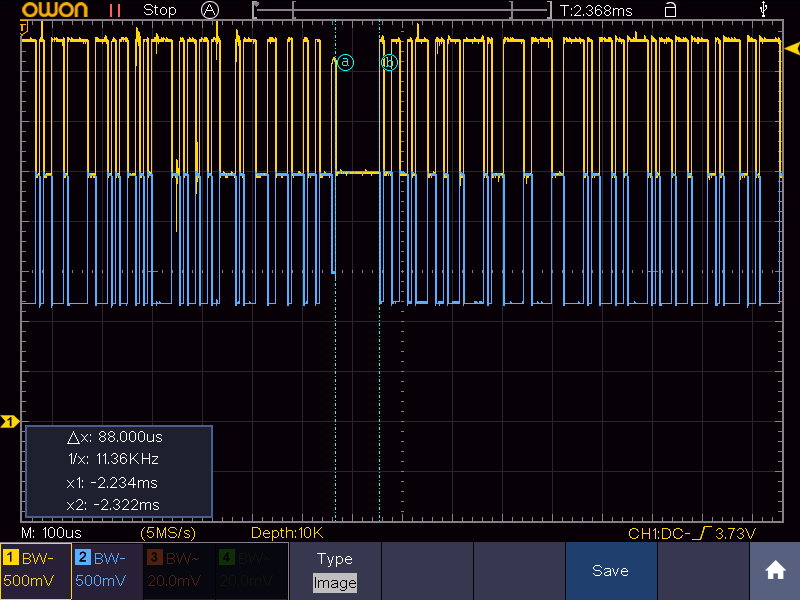
\includegraphics[width=1.0\linewidth]{1SNIP_SPROG_Interframe_2_900}
\caption{Interframe delay of SERVOIO-LCC reply.}
\label{fig:single_SERVOIO_SNIP_interframe}
\end{figure}
\cbend

\clearpage



\subsection{Double SNIP Interaction}

This measurement sends two SNIP requests sequentially and examines the timing of the replies.
This is intended to see what happens when a second request occurs before the first reply is sent.

The two request frames are sent at line rate, with no additional interframe time
between them.

In all four cases, the two SNIP requests were sent before the device sends the first 
SNIP reply frame.

The CS-105 and JMRI send their first responses with the delays typical of those seen 
above, and the second reply immediately after the first. 

In the single-SNIP measurement above, the Tower-LCC sent its reply in less than a single frame time
after the request was received.  
Here, the first reply frame follows the request with zero interframe time. 
The second reply frame, part of the first reply message, followed after
an interframe gap of typically 12-16\us.
See Figure \ref{fig:double_TWR_SNIP_interframe} for more detail on this.

The SERVOIO-LCC sent an OIR frame to temporarily reject the 2nd SNIP request
frame.
\footnote{The OpenLCB\textunderscore  Java library used by JMRI will 
    normally retransmit the SNIP request on receipt
    of a OIR addressed to it with a non-permanent error code; 
    what other control programs do is unknown at present.
}
See Figure \ref{fig:SERVOIO_double_SNIP_reply_sequence} for more detail on this.

To summarize, all four devices properly handled receiving a second SNIP request
message before the reply to the first request has been sent.


\begin{figure}[!htbp]
\centering
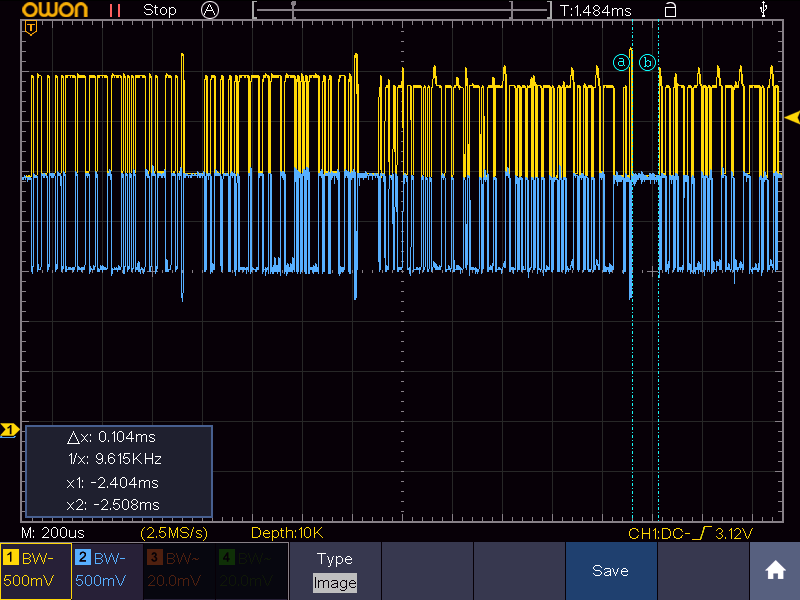
\includegraphics[width=1.0\linewidth]{2SNIP_TWR_Spacing}
\caption{Interframe delay of Tower-LCC SNIP reply with two requests.
The first two frames on the left are the SNIP requests sent to initiate the measurement.
The second two frames on the right are the SNIP reply from the Tower-LCC.
The interframe time between the first and second reply frame is measured at 16\us~here.
}
\label{fig:double_TWR_SNIP_interframe}
\end{figure}

\cbstart
\begin{figure}[!htbp]
\begin{verbatim}
03.662: [[19de8031] 08 1C                  ]  R: 03.00.00.00.00.01 - 02.01.2C.01.09.00 
                SimpleNodeIdentInfoRequest with no payload
03.663: [[19de8031] 08 1C                  ]  R: 03.00.00.00.00.01 - 02.01.2C.01.09.00
                SimpleNodeIdentInfoRequest with no payload
03.664: [[19a0881c] 10 31 04 53 50 52 4F 47]  R: SNIP Reply 1st frame
03.666: [[1906881c] 00 31 20 00 0D E8      ]  R: 02.01.2C.01.09.00 - 03.00.00.00.00.01 
                OptionalInteractionRejected with payload 20 00 0D E8 
                Optional Interaction Rejected for MTI 0xDE8 code 0x2000
03.666: [[19a0881c] 30 31 20 44 43 43 20 4C]  R: SNIP Reply middle frame
03.668: [[19a0881c] 30 31 74 64 00 53 45 52]  R: SNIP Reply middle frame
03.669: [[19a0881c] 30 31 56 4F 49 4F 2D 4C]  R: SNIP Reply middle frame
03.670: [[19a0881c] 30 31 43 43 00 31 2E 30]  R: SNIP Reply middle frame
03.671: [[19a0881c] 30 31 00 31 2E 35 00 02]  R: SNIP Reply middle frame
03.672: [[19a0881c] 20 31 00 00            ]  R: 02.01.2C.01.09.00 - 03.00.00.00.00.01 
                Simple Node Ident Info 
                with content '4,SPROG DCC Ltd,SERVOIO-LCC,1.0,1.5,2,,,'

\end{verbatim}
\caption{SERVOIO-LCC double-SNIP sequence. The SERVOIO-LCC starts to reply to the 1\ts{st}
        SNIP request, then sends a higher-priority OIR message to reject the
        2\ts{nd} request.}
\label{fig:SERVOIO_double_SNIP_reply_sequence}
\end{figure}
\cbend

\clearpage


\subsection{SNIP, PIP interaction}

This measurement sends a SNIP request followed by a higher-priority PIP request and 
examines the timing of the replies.
This is intended to see what happens when a second request with higher CAN priority occurs 
before the first reply can be sent.

The two request frames are sent at line rate, with no additional interframe time
between them.

The CS-105 replied to the PIP request before replying to the SNIP request. There were
no additional delays between the replies.

JMRI replied to first the SNIP request, then the PIP request with no additional
delays between the reply frames.

The Tower-LCC started its SNIP reply by sending the first frame, then replied to the 
PIP request, then sent the rest of the SNIP replies.  The interframe delays were 
typically 16\us.

The SERVOIO-LCC starts the SNIP reply with its first frame,
then sends the higher-priority PIP reply frame, 
followed by the rest of the SNIP reply frames.

\begin{figure}[!htbp]
\begin{verbatim}
50.187: [[19de8031] 03 00                  ]  R: 03.00.00.00.00.01 - 09.00.99.03.00.35 
    SimpleNodeIdentInfoRequest with no payload
50.187: [[19828031] 03 00                  ]  R: 03.00.00.00.00.01 - 09.00.99.03.00.35 
    ProtocolSupportInquiry with no payload
50.198: [[19668300] 00 31 54 58 00 00 00 00]  R: 09.00.99.03.00.35 - 03.00.00.00.00.01 
    ProtocolSupportReply with payload 54 58 00 00 00 00
50.199: [[19a08300] 10 31 04 54 72 61 69 6E]  R: SNIP Reply 1st frame
50.200: [[19a08300] 30 31 20 43 6F 6E 74 72]  R: SNIP Reply middle frame
50.201: [[19a08300] 30 31 6F 6C 20 53 79 73]  R: SNIP Reply middle frame
50.202: [[19a08300] 30 31 74 65 6D 73 20 28]  R: SNIP Reply middle frame
50.203: [[19a08300] 30 31 54 43 53 29 00 43]  R: SNIP Reply middle frame
50.204: [[19a08300] 30 31 53 2D 31 30 35 00]  R: SNIP Reply middle frame
50.206: [[19a08300] 30 31 52 65 76 20 45 00]  R: SNIP Reply middle frame
50.207: [[19a08300] 30 31 31 2E 30 30 00 02]  R: SNIP Reply middle frame
50.208: [[19a08300] 30 31 54 43 53 20 43 53]  R: SNIP Reply middle frame
50.209: [[19a08300] 30 31 2D 31 30 35 2C 20]  R: SNIP Reply middle frame
50.210: [[19a08300] 30 31 53 2F 4E 20 30 30]  R: SNIP Reply middle frame
50.211: [[19a08300] 30 31 33 35 00 54 43 53]  R: SNIP Reply middle frame
50.212: [[19a08300] 30 31 20 43 6F 6D 6D 61]  R: SNIP Reply middle frame
50.213: [[19a08300] 30 31 6E 64 20 53 74 61]  R: SNIP Reply middle frame
50.214: [[19a08300] 20 31 74 69 6F 6E 00   ]  R: 09.00.99.03.00.35 - 03.00.00.00.00.01 
    Simple Node Ident Info 
    with content '4,Train Control Systems (TCS),CS-105,Rev E,1.00,2,TCS CS-105, S/N 0035,TCS Command Station,'
\end{verbatim}
\caption{CS-105 SNIP, PIP reply packet sequence}
\label{fig:CS105_SNIP_PIP_reply_sequence}
\end{figure}

\begin{figure}[!htbp]
\begin{verbatim}
06.610: [[19de8031] 05 41                  ]  R: 03.00.00.00.00.01 - 02.01.57.00.04.9D 
    SimpleNodeIdentInfoRequest with no payload
06.611: [[19828031] 05 41                  ]  R: 03.00.00.00.00.01 - 02.01.57.00.04.9D 
    ProtocolSupportInquiry with no payload
06.612: [[19a08541] 10 31 04 52 52 2D 43 69]  R: SNIP Reply 1st frame
06.613: [[19668541] 00 31 D4 18 20 00 00 00]  R: 02.01.57.00.04.9D - 03.00.00.00.00.01 
    ProtocolSupportReply with payload D4 18 20 00 00 00
06.614: [[19a08541] 30 31 72 4B 69 74 73 2C]  R: SNIP Reply middle frame
06.615: [[19a08541] 30 31 20 49 6E 63 2E 00]  R: SNIP Reply middle frame
06.616: [[19a08541] 30 31 54 6F 77 65 72 2D]  R: SNIP Reply middle frame
06.617: [[19a08541] 30 31 4C 43 43 00 72 65]  R: SNIP Reply middle frame
06.618: [[19a08541] 30 31 76 2D 44 00 72 65]  R: SNIP Reply middle frame
06.619: [[19a08541] 30 31 76 2D 43 37 65 00]  R: SNIP Reply middle frame
06.620: [[19a08541] 30 31 02 5A 69 6F 6E 45]  R: SNIP Reply middle frame
06.621: [[19a08541] 30 31 20 74 75 72 6E 6F]  R: SNIP Reply middle frame
06.623: [[19a08541] 30 31 75 74 73 20 31 73]  R: SNIP Reply middle frame
06.624: [[19a08541] 30 31 74 20 32 34 2D 30]  R: SNIP Reply middle frame
06.625: [[19a08541] 30 31 31 2D 30 34 00 54]  R: SNIP Reply middle frame
06.626: [[19a08541] 30 31 75 72 6E 6F 75 74]  R: SNIP Reply middle frame
06.627: [[19a08541] 30 31 20 6F 77 6E 65 72]  R: SNIP Reply middle frame
06.628: [[19a08541] 20 31 2E 20 54 57 52 00]  R: 02.01.57.00.04.9D - 03.00.00.00.00.01 
    Simple Node Ident Info 
    with content '4,RR-CirKits, Inc.,Tower-LCC,rev-D,rev-C7e,2,ZionE turnouts 1st 24-01-04,Turnout owner. TWR,'
\end{verbatim}
\caption{TowerLCC SNIP, PIP reply packet sequence}
\label{fig:TWR_SNIP_PIP_reply_sequence}
\end{figure}

\cbstart
\begin{figure}[!htbp]
\begin{verbatim}
21.065: [[19de8031] 08 1C                  ]  R: 03.00.00.00.00.01 - 02.01.2C.01.09.00 
                SimpleNodeIdentInfoRequest with no payload
21.066: [[19828031] 08 1C                  ]  R: 03.00.00.00.00.01 - 02.01.2C.01.09.00 
                ProtocolSupportInquiry with no payload
21.067: [[19a0881c] 10 31 04 53 50 52 4F 47]  R: SNIP Reply 1st frame
21.069: [[1966881c] 00 31 54 58 20 00 00 00]  R: 02.01.2C.01.09.00 - 03.00.00.00.00.01 
                ProtocolSupportReply with payload 54 58 20 00 00 00
21.071: [[19a0881c] 30 31 20 44 43 43 20 4C]  R: SNIP Reply middle frame
21.071: [[19a0881c] 30 31 74 64 00 53 45 52]  R: SNIP Reply middle frame
21.072: [[19a0881c] 30 31 56 4F 49 4F 2D 4C]  R: SNIP Reply middle frame
21.073: [[19a0881c] 30 31 43 43 00 31 2E 30]  R: SNIP Reply middle frame
21.074: [[19a0881c] 30 31 00 31 2E 35 00 02]  R: SNIP Reply middle frame
21.075: [[19a0881c] 20 31 00 00            ]  R: 02.01.2C.01.09.00 - 03.00.00.00.00.01 
                Simple Node Ident Info 
                with content '4,SPROG DCC Ltd,SERVOIO-LCC,1.0,1.5,2,,,'
\end{verbatim}
\caption{SERVOIO-LCC SNIP, PIP reply packet sequence}
\label{fig:SERVOIO_SNIP_PIP_reply_sequence}
\end{figure}
\cbend

\clearpage

\subsection{Triple SNIP Interaction}

This measurement sends three SNIP requests sequentially and examines the timing of the replies.

Note that the SNIP request is lower priority than the SNIP reply. 
If a SNIP reply has already started by the time the third SNIP request is ready to send,
that request should be deferred from transmission until that reply has been completely sent.

For the CS-150 and JMRI PanelPro, there's enough delay before the first reply is 
sent that all three requests can go out.  
For these two devices, a delay has been added to schedule sending that 
3\ts{rd} SNIP request in the middle of the first SNIP reply.

In the case of the CS-105 and JMRI, 
the third SNIP request frame is delayed by CAN arbitration until after the
second SNIP reply message has been completely sent.

In the case of the Tower-LCC, the third SNIP request successfully arbitrates after the
first reply frame has been sent.  This is consistent with the Tower-LCC queuing the 
first frame of the reply while the second request is being sent so that it immediately
follows that second request, 
and then the third request successfully arbitrating during the extra
time that the Tower-LCC inserts between reply frames.

Note that the third SNIP request to the Tower-LCC is apparently
being lost, as there are only two SNIP replies.

In the case of the SERVOIO-LCC, the 2\ts{nd} and 3\ts{rd}
SNIP requests get an OIR temporarily rejecting them.

\begin{figure}[!htbp]
\begin{verbatim}
35.218: [[19de8031] 03 00                  ]  R: 03.00.00.00.00.01 - 09.00.99.03.00.35 
    SimpleNodeIdentInfoRequest with no payload
35.223: [[19de8031] 03 00                  ]  R: 03.00.00.00.00.01 - 09.00.99.03.00.35 
    SimpleNodeIdentInfoRequest with no payload
35.230: [[19a08300] 10 31 04 54 72 61 69 6E]  R: SNIP Reply 1st frame
35.238: [[19a08300] 30 31 20 43 6F 6E 74 72]  R: SNIP Reply middle frame
35.238: [[19a08300] 30 31 6F 6C 20 53 79 73]  R: SNIP Reply middle frame
35.238: [[19a08300] 30 31 74 65 6D 73 20 28]  R: SNIP Reply middle frame
35.238: [[19a08300] 30 31 54 43 53 29 00 43]  R: SNIP Reply middle frame
35.238: [[19a08300] 30 31 53 2D 31 30 35 00]  R: SNIP Reply middle frame
35.238: [[19a08300] 30 31 52 65 76 20 45 00]  R: SNIP Reply middle frame
35.238: [[19a08300] 30 31 31 2E 30 30 00 02]  R: SNIP Reply middle frame
35.239: [[19a08300] 30 31 54 43 53 20 43 53]  R: SNIP Reply middle frame
35.242: [[19a08300] 30 31 2D 31 30 35 2C 20]  R: SNIP Reply middle frame
35.242: [[19a08300] 30 31 53 2F 4E 20 30 30]  R: SNIP Reply middle frame
35.242: [[19a08300] 30 31 33 35 00 54 43 53]  R: SNIP Reply middle frame
35.255: [[19a08300] 30 31 20 43 6F 6D 6D 61]  R: SNIP Reply middle frame
35.255: [[19a08300] 30 31 6E 64 20 53 74 61]  R: SNIP Reply middle frame
35.255: [[19a08300] 20 31 74 69 6F 6E 00   ]  R: 09.00.99.03.00.35 - 03.00.00.00.00.01 
    Simple Node Ident Info with content '4,Train Control Systems (TCS),CS-105,Rev E,1.00,2,TCS CS-105, S/N 0035,TCS Command Station,'
35.255: [[19a08300] 10 31 04 54 72 61 69 6E]  R: SNIP Reply 1st frame
35.255: [[19a08300] 30 31 20 43 6F 6E 74 72]  R: SNIP Reply middle frame
35.255: [[19a08300] 30 31 6F 6C 20 53 79 73]  R: SNIP Reply middle frame
35.255: [[19a08300] 30 31 74 65 6D 73 20 28]  R: SNIP Reply middle frame
...
35.271: [[19a08300] 30 31 20 43 6F 6D 6D 61]  R: SNIP Reply middle frame
35.271: [[19a08300] 30 31 6E 64 20 53 74 61]  R: SNIP Reply middle frame
35.271: [[19a08300] 20 31 74 69 6F 6E 00   ]  R: 09.00.99.03.00.35 - 03.00.00.00.00.01 
    Simple Node Ident Info with content '4,Train Control Systems (TCS),CS-105,Rev E,1.00,2,TCS CS-105, S/N 0035,TCS Command Station,'
35.271: [[19de8031] 03 00                  ]  R: 03.00.00.00.00.01 - 09.00.99.03.00.35 
    SimpleNodeIdentInfoRequest with no payload
35.274: [[19a08300] 10 31 04 54 72 61 69 6E]  R: SNIP Reply 1st frame
35.286: [[19a08300] 30 31 20 43 6F 6E 74 72]  R: SNIP Reply middle frame
35.286: [[19a08300] 30 31 6F 6C 20 53 79 73]  R: SNIP Reply middle frame
...
35.290: [[19a08300] 30 31 20 43 6F 6D 6D 61]  R: SNIP Reply middle frame
35.290: [[19a08300] 30 31 6E 64 20 53 74 61]  R: SNIP Reply middle frame
35.290: [[19a08300] 20 31 74 69 6F 6E 00   ]  R: 09.00.99.03.00.35 - 03.00.00.00.00.01 
    Simple Node Ident Info with content '4,Train Control Systems (TCS),CS-105,Rev E,1.00,2,TCS CS-105, S/N 0035,TCS Command Station,'
\end{verbatim}
\caption{CS-105 triple SNIP reply packet sequence.
Note: Some SNIP Reply middle frames elided to save space.}
\label{fig:CS105_Triple_SNIP_reply_sequence}
\end{figure}


\begin{figure}[!htbp]
\begin{verbatim}
18.722: [[19de8031] 05 41                  ]  R: 03.00.00.00.00.01 - 02.01.57.00.04.9D 
    SimpleNodeIdentInfoRequest with no payload
18.723: [[19de8031] 05 41                  ]  R: 03.00.00.00.00.01 - 02.01.57.00.04.9D 
    SimpleNodeIdentInfoRequest with no payload
18.724: [[19a08541] 10 31 04 52 52 2D 43 69]  R: SNIP Reply 1st frame
18.725: [[19de8031] 05 41                  ]  R: 03.00.00.00.00.01 - 02.01.57.00.04.9D
    SimpleNodeIdentInfoRequest with no payload
18.726: [[19a08541] 30 31 72 4B 69 74 73 2C]  R: SNIP Reply middle frame
18.727: [[19a08541] 30 31 20 49 6E 63 2E 00]  R: SNIP Reply middle frame
18.728: [[19a08541] 30 31 54 6F 77 65 72 2D]  R: SNIP Reply middle frame
18.729: [[19a08541] 30 31 4C 43 43 00 72 65]  R: SNIP Reply middle frame
18.730: [[19a08541] 30 31 76 2D 44 00 72 65]  R: SNIP Reply middle frame
18.731: [[19a08541] 30 31 76 2D 43 37 65 00]  R: SNIP Reply middle frame
18.733: [[19a08541] 30 31 02 5A 69 6F 6E 45]  R: SNIP Reply middle frame
18.734: [[19a08541] 30 31 20 74 75 72 6E 6F]  R: SNIP Reply middle frame
18.735: [[19a08541] 30 31 75 74 73 20 31 73]  R: SNIP Reply middle frame
18.736: [[19a08541] 30 31 74 20 32 34 2D 30]  R: SNIP Reply middle frame
18.737: [[19a08541] 30 31 31 2D 30 34 00 54]  R: SNIP Reply middle frame
18.738: [[19a08541] 30 31 75 72 6E 6F 75 74]  R: SNIP Reply middle frame
18.739: [[19a08541] 30 31 20 6F 77 6E 65 72]  R: SNIP Reply middle frame
18.740: [[19a08541] 20 31 2E 20 54 57 52 00]  R: 02.01.57.00.04.9D - 03.00.00.00.00.01 
    Simple Node Ident Info with content '4,RR-CirKits, Inc.,Tower-LCC,rev-D,rev-C7e,2,ZionE turnouts 1st 24-01-04,Turnout owner. TWR,'
18.742: [[19a08541] 10 31 04 52 52 2D 43 69]  R: SNIP Reply 1st frame
18.743: [[19a08541] 30 31 72 4B 69 74 73 2C]  R: SNIP Reply middle frame
18.744: [[19a08541] 30 31 20 49 6E 63 2E 00]  R: SNIP Reply middle frame
18.745: [[19a08541] 30 31 54 6F 77 65 72 2D]  R: SNIP Reply middle frame
18.746: [[19a08541] 30 31 4C 43 43 00 72 65]  R: SNIP Reply middle frame
18.747: [[19a08541] 30 31 76 2D 44 00 72 65]  R: SNIP Reply middle frame
18.748: [[19a08541] 30 31 76 2D 43 37 65 00]  R: SNIP Reply middle frame
18.749: [[19a08541] 30 31 02 5A 69 6F 6E 45]  R: SNIP Reply middle frame
18.750: [[19a08541] 30 31 20 74 75 72 6E 6F]  R: SNIP Reply middle frame
18.751: [[19a08541] 30 31 75 74 73 20 31 73]  R: SNIP Reply middle frame
18.752: [[19a08541] 30 31 74 20 32 34 2D 30]  R: SNIP Reply middle frame
18.754: [[19a08541] 30 31 31 2D 30 34 00 54]  R: SNIP Reply middle frame
18.755: [[19a08541] 30 31 75 72 6E 6F 75 74]  R: SNIP Reply middle frame
18.756: [[19a08541] 30 31 20 6F 77 6E 65 72]  R: SNIP Reply middle frame
18.757: [[19a08541] 20 31 2E 20 54 57 52 00]  R: 02.01.57.00.04.9D - 03.00.00.00.00.01 
    Simple Node Ident Info with content '4,RR-CirKits, Inc.,Tower-LCC,rev-D,rev-C7e,2,ZionE turnouts 1st 24-01-04,Turnout owner. TWR,'
\end{verbatim}
\caption{TowerLCC triple SNIP reply packet sequence.
Note that there is no reply to the third SNIP request.}
\label{fig:TWR_Triple_SNIP_reply_sequence}
\end{figure}

\cbstart
\begin{figure}[!htbp]
\begin{verbatim}
02.120: [[19de8031] 08 1C                  ]  R: 03.00.00.00.00.01 - 02.01.2C.01.09.00 
                SimpleNodeIdentInfoRequest with no payload
02.120: [[19de8031] 08 1C                  ]  R: 03.00.00.00.00.01 - 02.01.2C.01.09.00 
                SimpleNodeIdentInfoRequest with no payload
02.121: [[19de8031] 08 1C                  ]  R: 03.00.00.00.00.01 - 02.01.2C.01.09.00 
                SimpleNodeIdentInfoRequest with no payload
02.123: [[19a0881c] 10 31 04 53 50 52 4F 47]  R: SNIP Reply 1st frame
02.123: [[1906881c] 00 31 20 00 0D E8      ]  R: 02.01.2C.01.09.00 - 03.00.00.00.00.01 
                OptionalInteractionRejected with payload 20 00 0D E8 
                Optional Interaction Rejected for MTI 0xDE8 code 0x2000
02.125: [[19a0881c] 30 31 20 44 43 43 20 4C]  R: SNIP Reply middle frame
02.126: [[1906881c] 00 31 20 00 0D E8      ]  R: 02.01.2C.01.09.00 - 03.00.00.00.00.01 
                OptionalInteractionRejected with payload 20 00 0D E8 
                Optional Interaction Rejected for MTI 0xDE8 code 0x2000
02.126: [[19a0881c] 30 31 74 64 00 53 45 52]  R: SNIP Reply middle frame
02.128: [[19a0881c] 30 31 56 4F 49 4F 2D 4C]  R: SNIP Reply middle frame
02.129: [[19a0881c] 30 31 43 43 00 31 2E 30]  R: SNIP Reply middle frame
02.130: [[19a0881c] 30 31 00 31 2E 35 00 02]  R: SNIP Reply middle frame
02.131: [[19a0881c] 20 31 00 00            ]  R: 02.01.2C.01.09.00 - 03.00.00.00.00.01 
                Simple Node Ident Info with content '4,SPROG DCC Ltd,SERVOIO-LCC,1.0,1.5,2,,,'
\end{verbatim}
\caption{SERVOIO-LCC triple SNIP reply packet sequence.
Note that the 2nd two requests receive OIR replies}
\label{fig:SERVOIO_Triple_SNIP_reply_sequence}
\end{figure}
\cbend





\clearpage

\subsection{SNIP, SNIP, PIP Interaction}

This measurement sequentially sends two SNIP requests followed by a higher-priority PIP request
and examines the timing of the replies.

This is similar to the Triple SNIP interaction examined above, except that
the third request is of higher CAN priority than the first two.

For the CS-150 and JMRI PanelPro, there's enough delay before the first reply is 
sent that all three requests can go out.  
For these two devices, a delay has been added to schedule sending that 
request in the middle of the first SNIP reply.

For all four devices,  
the PIP request successfully arbitrates immediately, appearing during the 
SNIP reply sequence. 

For the CS-105 and JMRI,
the PIP reply is delayed until after the two SNIP replies are complete.

Note that the 2nd SNIP request to the Tower-LCC is apparently
being lost, as there is only one SNIP reply.

The SERVOIO-LCC interleaves its OIR reply to the 2\ts{nd} SNIP request
with the start of the 1\ts{st} SNIP reply, followed by the PIP reply 
a frame later.
See Figure \ref{fig:SERVOIO_SNIP2PIP_reply_sequence} for more detail on this.


\begin{figure}[!htbp]
\begin{verbatim}
37.595: [[19de8031] 03 00                  ]  R: 03.00.00.00.00.01 - 09.00.99.03.00.35
    SimpleNodeIdentInfoRequest with no payload
37.596: [[19de8031] 03 00                  ]  R: 03.00.00.00.00.01 - 09.00.99.03.00.35
    SimpleNodeIdentInfoRequest with no payload
37.607: [[19a08300] 10 31 04 54 72 61 69 6E]  R: SNIP Reply 1st frame
37.608: [[19a08300] 30 31 20 43 6F 6E 74 72]  R: SNIP Reply middle frame
37.609: [[19a08300] 30 31 6F 6C 20 53 79 73]  R: SNIP Reply middle frame
37.610: [[19a08300] 30 31 74 65 6D 73 20 28]  R: SNIP Reply middle frame
37.611: [[19a08300] 30 31 54 43 53 29 00 43]  R: SNIP Reply middle frame
37.613: [[19a08300] 30 31 53 2D 31 30 35 00]  R: SNIP Reply middle frame
37.614: [[19a08300] 30 31 52 65 76 20 45 00]  R: SNIP Reply middle frame
37.614: [[19828031] 03 00                  ]  R: 03.00.00.00.00.01 - 09.00.99.03.00.35
    ProtocolSupportInquiry with no payload
37.615: [[19a08300] 30 31 31 2E 30 30 00 02]  R: SNIP Reply middle frame
37.617: [[19a08300] 30 31 54 43 53 20 43 53]  R: SNIP Reply middle frame
37.618: [[19a08300] 30 31 2D 31 30 35 2C 20]  R: SNIP Reply middle frame
37.619: [[19a08300] 30 31 53 2F 4E 20 30 30]  R: SNIP Reply middle frame
37.621: [[19a08300] 30 31 33 35 00 54 43 53]  R: SNIP Reply middle frame
37.621: [[19a08300] 30 31 20 43 6F 6D 6D 61]  R: SNIP Reply middle frame
37.623: [[19a08300] 30 31 6E 64 20 53 74 61]  R: SNIP Reply middle frame
37.624: [[19a08300] 20 31 74 69 6F 6E 00   ]  R: 09.00.99.03.00.35 - 03.00.00.00.00.01
    Simple Node Ident Info with content '4,Train Control Systems (TCS),CS-105,Rev E,1.00,2,TCS CS-105, S/N 0035,TCS Command Station,'
37.625: [[19a08300] 10 31 04 54 72 61 69 6E]  R: SNIP Reply 1st frame
37.626: [[19a08300] 30 31 20 43 6F 6E 74 72]  R: SNIP Reply middle frame
37.627: [[19a08300] 30 31 6F 6C 20 53 79 73]  R: SNIP Reply middle frame
37.628: [[19a08300] 30 31 74 65 6D 73 20 28]  R: SNIP Reply middle frame
37.630: [[19a08300] 30 31 54 43 53 29 00 43]  R: SNIP Reply middle frame
37.631: [[19a08300] 30 31 53 2D 31 30 35 00]  R: SNIP Reply middle frame
37.632: [[19a08300] 30 31 52 65 76 20 45 00]  R: SNIP Reply middle frame
37.634: [[19a08300] 30 31 31 2E 30 30 00 02]  R: SNIP Reply middle frame
37.634: [[19a08300] 30 31 54 43 53 20 43 53]  R: SNIP Reply middle frame
37.635: [[19a08300] 30 31 2D 31 30 35 2C 20]  R: SNIP Reply middle frame
37.636: [[19a08300] 30 31 53 2F 4E 20 30 30]  R: SNIP Reply middle frame
37.637: [[19a08300] 30 31 33 35 00 54 43 53]  R: SNIP Reply middle frame
37.638: [[19a08300] 30 31 20 43 6F 6D 6D 61]  R: SNIP Reply middle frame
37.639: [[19a08300] 30 31 6E 64 20 53 74 61]  R: SNIP Reply middle frame
37.640: [[19a08300] 20 31 74 69 6F 6E 00   ]  R: 09.00.99.03.00.35 - 03.00.00.00.00.01 
    Simple Node Ident Info with content '4,Train Control Systems (TCS),CS-105,Rev E,1.00,2,TCS CS-105, S/N 0035,TCS Command Station,'
37.641: [[19668300] 00 31 54 58 00 00 00 00]  R: 09.00.99.03.00.35 - 03.00.00.00.00.01 
    ProtocolSupportReply with payload 54 58 00 00 00 00
\end{verbatim}
\caption{CS-105 SNIP, SNIP, PIP reply packet sequence.}
\label{fig:CS105_SNIP2PIP_reply_sequence}
\end{figure}


\begin{figure}[!htbp]
\begin{verbatim}
05.502: [[19de8031] 0A 20                  ]  R: 03.00.00.00.00.01 - 02.01.12.FE.E6.6D 
    SimpleNodeIdentInfoRequest with no payload
05.503: [[19de8031] 0A 20                  ]  R: 03.00.00.00.00.01 - 02.01.12.FE.E6.6D 
    SimpleNodeIdentInfoRequest with no payload
05.504: [[19a08a20] 10 31 04 4A 4D 52 49 00]  R: SNIP Reply 1st frame
05.505: [[19a08a20] 30 31 50 61 6E 65 6C 50]  R: SNIP Reply middle frame
05.506: [[19a08a20] 30 31 72 6F 00 4D 79 20]  R: SNIP Reply middle frame
05.507: [[19a08a20] 30 31 4A 4D 52 49 20 52]  R: SNIP Reply middle frame
05.508: [[19a08a20] 30 31 61 69 6C 72 6F 61]  R: SNIP Reply middle frame
05.509: [[19828031] 0A 20                  ]  R: 03.00.00.00.00.01 - 02.01.12.FE.E6.6D 
    ProtocolSupportInquiry with no payload
05.510: [[19a08a20] 30 31 64 00 35 2E 37 2E]  R: SNIP Reply middle frame
05.511: [[19a08a20] 30 31 34 70 6C 75 73 2B]  R: SNIP Reply middle frame
05.512: [[19a08a20] 30 31 6A 61 6B 65 2B 32]  R: SNIP Reply middle frame
05.513: [[19a08a20] 30 31 30 32 34 30 00 02]  R: SNIP Reply middle frame
05.514: [[19a08a20] 20 31 00 00            ]  R: 02.01.12.FE.E6.6D - 03.00.00.00.00.01 
    Simple Node Ident Info with content '4,JMRI,PanelPro,My JMRI Railroad,5.7.4plus+jake+20240,2,,,'
05.515: [[19a08a20] 10 31 04 4A 4D 52 49 00]  R: SNIP Reply 1st frame
05.516: [[19a08a20] 30 31 50 61 6E 65 6C 50]  R: SNIP Reply middle frame
05.517: [[19a08a20] 30 31 72 6F 00 4D 79 20]  R: SNIP Reply middle frame
05.518: [[19a08a20] 30 31 4A 4D 52 49 20 52]  R: SNIP Reply middle frame
05.519: [[19a08a20] 30 31 61 69 6C 72 6F 61]  R: SNIP Reply middle frame
05.520: [[19a08a20] 30 31 64 00 35 2E 37 2E]  R: SNIP Reply middle frame
05.521: [[19a08a20] 30 31 34 70 6C 75 73 2B]  R: SNIP Reply middle frame
05.523: [[19a08a20] 30 31 6A 61 6B 65 2B 32]  R: SNIP Reply middle frame
05.524: [[19a08a20] 30 31 30 32 34 30 00 02]  R: SNIP Reply middle frame
05.524: [[19a08a20] 20 31 00 00            ]  R: 02.01.12.FE.E6.6D - 03.00.00.00.00.01 
    Simple Node Ident Info with content '4,JMRI,PanelPro,My JMRI Railroad,5.7.4plus+jake+20240,2,,,'
05.526: [[19668a20] 00 31 04 10 00 00 00 00]  R: 02.01.12.FE.E6.6D - 03.00.00.00.00.01 
    ProtocolSupportReply with payload 04 10 00 00 00 00
\end{verbatim}
\caption{JMRI SNIP, SNIP, PIP reply packet sequence.}
\label{fig:JMRI_SNIP2PIP_reply_sequence}
\end{figure}


\begin{figure}[!htbp]
\begin{verbatim}
45.836: [[19de8031] 05 41                  ]  R: 03.00.00.00.00.01 - 02.01.57.00.04.9D 
    SimpleNodeIdentInfoRequest with no payload
45.837: [[19de8031] 05 41                  ]  R: 03.00.00.00.00.01 - 02.01.57.00.04.9D 
    SimpleNodeIdentInfoRequest with no payload
45.838: [[19828031] 05 41                  ]  R: 03.00.00.00.00.01 - 02.01.57.00.04.9D 
    ProtocolSupportInquiry with no payload
45.839: [[19a08541] 10 31 04 52 52 2D 43 69]  R: SNIP Reply 1st frame
45.840: [[19668541] 00 31 D4 18 20 00 00 00]  R: 02.01.57.00.04.9D - 03.00.00.00.00.01 
    ProtocolSupportReply with payload D4 18 20 00 00 00
45.841: [[19a08541] 30 31 72 4B 69 74 73 2C]  R: SNIP Reply middle frame
45.842: [[19a08541] 30 31 20 49 6E 63 2E 00]  R: SNIP Reply middle frame
45.843: [[19a08541] 30 31 54 6F 77 65 72 2D]  R: SNIP Reply middle frame
45.844: [[19a08541] 30 31 4C 43 43 00 72 65]  R: SNIP Reply middle frame
45.846: [[19a08541] 30 31 76 2D 44 00 72 65]  R: SNIP Reply middle frame
45.847: [[19a08541] 30 31 76 2D 43 37 65 00]  R: SNIP Reply middle frame
45.848: [[19a08541] 30 31 02 5A 69 6F 6E 45]  R: SNIP Reply middle frame
45.849: [[19a08541] 30 31 20 74 75 72 6E 6F]  R: SNIP Reply middle frame
45.850: [[19a08541] 30 31 75 74 73 20 31 73]  R: SNIP Reply middle frame
45.851: [[19a08541] 30 31 74 20 32 34 2D 30]  R: SNIP Reply middle frame
45.852: [[19a08541] 30 31 31 2D 30 34 00 54]  R: SNIP Reply middle frame
45.853: [[19a08541] 30 31 75 72 6E 6F 75 74]  R: SNIP Reply middle frame
45.854: [[19a08541] 30 31 20 6F 77 6E 65 72]  R: SNIP Reply middle frame
45.856: [[19a08541] 20 31 2E 20 54 57 52 00]  R: 02.01.57.00.04.9D - 03.00.00.00.00.01 
    Simple Node Ident Info with content '4,RR-CirKits, Inc.,Tower-LCC,rev-D,rev-C7e,2,ZionE turnouts 1st 24-01-04,Turnout owner. TWR,'
\end{verbatim}
\caption{TowerLCC SNIP, SNIP, PIP reply packet sequence.}
\label{fig:TWR_SNIP2PIP_reply_sequence}
\end{figure}

\cbstart
\begin{figure}[!htbp]
\begin{verbatim}
37.712: [[19de8031] 08 1C                  ]  R: 03.00.00.00.00.01 - 02.01.2C.01.09.00 
                SimpleNodeIdentInfoRequest with no payload
37.713: [[19de8031] 08 1C                  ]  R: 03.00.00.00.00.01 - 02.01.2C.01.09.00 
                SimpleNodeIdentInfoRequest with no payload
37.714: [[19828031] 08 1C                  ]  R: 03.00.00.00.00.01 - 02.01.2C.01.09.00 
                ProtocolSupportInquiry with no payload
37.715: [[19a0881c] 10 31 04 53 50 52 4F 47]  R: SNIP Reply 1st frame
37.716: [[1906881c] 00 31 20 00 0D E8      ]  R: 02.01.2C.01.09.00 - 03.00.00.00.00.01 
                OptionalInteractionRejected with payload 20 00 0D E8 
                Optional Interaction Rejected for MTI 0xDE8 code 0x2000
37.717: [[19a0881c] 30 31 20 44 43 43 20 4C]  R: SNIP Reply middle frame
37.718: [[1966881c] 00 31 54 58 20 00 00 00]  R: 02.01.2C.01.09.00 - 03.00.00.00.00.01 
                ProtocolSupportReply with payload 54 58 20 00 00 00
37.719: [[19a0881c] 30 31 74 64 00 53 45 52]  R: SNIP Reply middle frame
37.720: [[19a0881c] 30 31 56 4F 49 4F 2D 4C]  R: SNIP Reply middle frame
37.721: [[19a0881c] 30 31 43 43 00 31 2E 30]  R: SNIP Reply middle frame
37.722: [[19a0881c] 30 31 00 31 2E 35 00 02]  R: SNIP Reply middle frame
37.723: [[19a0881c] 20 31 00 00            ]  R: 02.01.2C.01.09.00 - 03.00.00.00.00.01 
                Simple Node Ident Info 
                with content '4,SPROG DCC Ltd,SERVOIO-LCC,1.0,1.5,2,,,'
\end{verbatim}
\caption{SERVOIO-LCC SNIP, SNIP, PIP reply packet sequence.}
\label{fig:SERVOIO_SNIP2PIP_reply_sequence}
\end{figure}
\cbend

\clearpage

\section{Summary}

The TCS CS-105 and JMRI PanelPro with LCC Buffer-USB have millisecond-scale delays between receipt
of a request and the start of a reply, which can allow additional requests to arrive
before the first reply is sent.  
Both of these rely on deep buffers to handle this.
They both send the frames of an individual reply
at line speed, preventing a lower-priority request from arriving during the reply.

The RR-CirKits Tower-LCC replies in less than one frame time, allowing only one additional
request to arrive before the reply starts.  It has short additional delays
between the frames of the response, which can allow lower priority
requests to arrive and need buffer space during the reply.  
In the extremely unlikely case of three requests arriving within a few milliseconds, one
of them would be lost.

\cbstart
The SPROG DCC Ltd. SERVOIO-LCC replies about 0.6 to 1.0 milliseconds after receipt of a 
request.  
It sends the frames of an individual reply
at line speed, preventing a lower-priority request from arriving during the reply.
\cbend
Instead of buffering multiple SNIP requests, the SERVOIO-LCC rejects additional
overlapping SNIP requests with an 
Optional Interaction Rejected (OIR) message that 
should trigger a retry of the interaction.


The implications of this for the Events-with-Payload protocol update need to be 
examined carefully.

\end{document}
